\subsubsection{Verify the ($k-\omega$) barrier coverage}
The problem is formulated as follows. Given a set of $n$ sensors $S=\{S_1,S_2,...,S_n\}$ and a rectangular region $\Omega$ with the length of $L$ and the width of $W$. $\Omega$ is called the monitoring region and camera sensors in $S$ are deployed according to uniform deployment scheme in $\Omega$ to serve the purpose of observation. The uniform deployment scheme means that total $ n $ sensors are deployed randomly, uniformly and independently.\par

The objective of the problem is to verify if $\Omega$ achieves multiple-view barrier coverage. In other words, we need to determine if there exists a multiple-view barrier $B$ in $\Omega$. If there is none, $\Omega$ will not guarantee security requirements and the sensors need to be re-deployed.\par

Unlike omni-directional sensor, which only provides information about detection of the object, camera sensor is typically directional sensor and can be used to obtain multimedia information of the object. Each camera sensor can be denoted by a 4-tuple $\{S_i, R, \alpha, \varphi_i\}$, where $S_i$ is the location of sensor $i$, $R$ is the sensing radius and $\alpha$ is half of the sensing angle. We assume that all sensors have the same sensing radius and sensing angle. In reality, sensing range of camera sensor is usually less than $\pi$, so we also have an assumption that $\alpha < \displaystyle\frac{\pi}{2}$. The last parameter of a camera sensor, $\varphi_i$, is the facing direction of sensor $i$, which is uniformly distributed in $[0,2\pi]$ \par
Figure \ref{sensing-model} shows information of sensor $s$.
\begin{figure}[h]
	\centering
	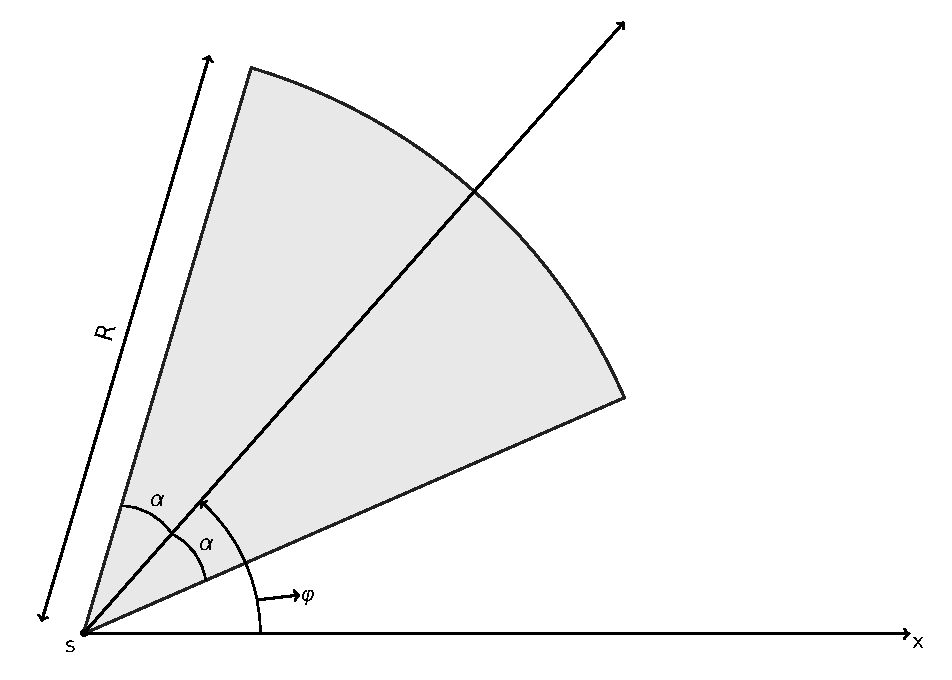
\includegraphics[scale=.7]{Hinhanh/sensing-model}
	\caption{Illustration of a camera sensor $s$. The shadow area is the sensing region of $s$}
	\label{sensing-model}
\end{figure}

\noindent The input and output of the problem are followings:\\[7pt]
{\bfseries Input}
\begin{itemize}
	\item $L, W$: Length and width of the monitoring region $\Omega$ respectively.
	\item $n$: Number of camera sensors.
	\item $S = \{S_1,S_2,...,S_n\}$: Set of camera sensors. $S_i$ denotes the $i$-th camera sensor and also denotes the location of that sensor.
	\item $R$: Radius of camera sensors.
	\item $\alpha$: Half of the sensing angle of camera sensors.
	\item $\varphi_i$: Orientation angle view of $S_i$ where $i=\overline{1,n}$.
	\item $k, \omega$ : The conditional parameter of the problem.
\end{itemize}
{\bfseries Output}
\begin{itemize}
	\item The yes/no answer that the monitoring region achieves multiple-view barrier coverage. 
\end{itemize}

\subsubsection{Evaluate the quality of a multiple-view barrier}
The problem is formulated as follows. Given a barrier $B$ in a sensing field containing several connected regions $B_i$ from the left to the right boundary of the field. Each $B_i$ is a closing field that is ($k-\omega$) covered by a $k$-list of sensors $P_i$.

The objective of the problem is to find the coverage of the barrier regarding our devised metric. The process is to assess the quality of the found barrier and compare the result with other settings of parameters to analyze the effect of each parameter to the quality of the sensing field and find the best combination of settings to achieve our desire.

\noindent The input and output of the problem are followings:\\[7pt]
{\bfseries Input}
\begin{itemize}
	\item $\{B_i\}$: The set of closing region connect the left and the right edge of the sensing field.
	\item $\{P_i\}$: The set of $k$-list of sensors, the $P_i$ is known to ($k,\omega$) cover the region $B_i$.
\end{itemize}
{\bfseries Output}
\begin{itemize}
	\item The coverage value of the ($k,\omega$) barrier.
\end{itemize}